%
% sinh.tex -- warum sinh und cosh für gewöhnliche DGl so nützlich sind
%
% (c) 2015 Prof Dr Andreas Müller, Hochschule Rapperswil
%
\chapter{Hyperbolische Funktionen}
Das Standardverfahren f"ur die L"osung linearer Differentialgleichungen
mit konstanter Koeffizienten liefert typischerweise Schwingungsl"osungen
oder exponentiell abfallende oder anwachsende L"osungen. Die Koeffizienten
der allgemeinen L"osungen m"ussen dann mit Hilfe der Anfangswerte bestimmt
werden. F"ur die Schwingunsgl"osungen ist das meist sehr viel einfacher
als f"ur die exponentiellen L"osungen. Hier wird gezeigt, wie man mit
Hilfe der hyperbolischen Funktionen die L"osungen ebenso einfach ausdr"ucken
kann.

\section{Differentialgleichungen zweiter Ordnung}
Das Standardverfahren f"ur die L"osung einer gew"ohnlichen linearen
Differentialgleichung mit konstanten Koeffizienten
\[
a_2y''+ a_1y'+a_0y=0
\]
schreibt vor, dass man erst die Nullstellen $\lambda_{1,2}$
des charakteristischen Polynoms
\[
p(\lambda)=a_2\lambda^2+a_1\lambda+a_0
\]
finden muss.
Die allgemeine L"osung der Differentialgleichung ist dann
eine Linearkombination
\[
y(x)=
A_1 e^{\lambda_1t}
+
A_2 e^{\lambda_2t},
\]
die Konstanten $A_1$ und $A_2$ sind aus den Anfangswerten zu bestimmen.
Sinde $y_0$ und $v_0$ der Anfangswert und die Anfangsableitung, dann
findet man das lineare Gleichungssystem
%\newcolumntype{\linsysR}{>{$}r<{$}}
%\newcolumntype{\linsysL}{>{$}l<{$}}
%\newcolumntype{\linsysC}{>{$}c<{$}}
%\newenvironment{linsys}[1]{%
%\begin{tabular}{*{#1}{\linsysR@{\;}\linsysC}@{\;}\linsysR}}%
%{\end{tabular}}
\[
\begin{linsys}{3}
         A_1&+&         A_2&=&y_0\phantom{.}\\
\lambda_1A_1&+&\lambda_2A_2&=&v_0.
\end{linsys}
\]
Besonders einfach wird die Bestimmung jedoch f"ur die Differentialgleichung
\[
y''+k^2 y=0.
\]
Dann sind die $\lambda_{1,2}=\pm\sqrt{-k^2}$ imagin"ar, und man kann statt
der Exponentiall"osungen auch den Ansatz
\[
y(x)=A\cos kx+B\sin kx
\]
verwenden.
Da der Wert von $\sin kx$ bei $x=0$ verschwindet, und die Ableitung von
$\cos kx$ ebenfalls, ist die Bestimmung der Konstanten viel einfacher:
\[
A=y_0
\qquad\text{und}\qquad
B=\frac1kv_0,
\]
oder
\begin{equation}
y(x)=y_0\cos kx + \frac{v_0}{k}\sin kx
\label{hyp:loesung}
\end{equation}

F"ur die analoge Differentialgleichung $y''-k^2y=0$ geht dies nicht.
Die Nullstellen des charakteristischen Polynoms sind hier 
$\lambda_{1,2}=\pm k$, und es f"uhrt nichts an dem linearen Gleichungssystem
\[
\begin{linsys}{3}
 A_1&+& A_2&=&y_0\\
kA_1&-&kA_2&=&v_0
\end{linsys}
\]
vorbei.
Die L"osung kann allerdings zum Beispiel mit dem Determinantenverfahren
ziemlich direkt gefunden werden:
\[
\begin{aligned}
A_1
&=
\frac{\left|\begin{matrix}y_0&1\\v_0&-k\end{matrix}\right|}{\left|\begin{matrix}1&1\\k&-k\end{matrix}\right|}
=
\frac{-ky_0+v_0}{-2k},
&
&&
A_2
&=
\frac{\left|\begin{matrix}1&y_0\\k&v_0\end{matrix}\right|}{\left|\begin{matrix}1&1\\k&-k\end{matrix}\right|}
=\frac{v_0-ky_0}{-2k}.
\end{aligned}
\]
Damit kann man jetzt die L"osung auch in diesem Fall hinschreiben:
\begin{align}
y(x)
&=
A_1e^{kx}+A_2e^{-kx}
=
\frac12\biggl(
\frac{ky_0-v_0}k e^{kx}
+
\frac{-v_0+ky_0}k e^{-kx}
\biggr)
\notag
\\
&=
y_0\frac{e^{kx}+e^{-kx}}2
+\frac{v_0}{k}\frac{e^{kx}-e^{-kx}}2.
\label{hyp:hyperbelfunktionen}
\end{align}
Die Erf"ullung der Anfangsbedingung k"onnte also auch in diesem Falle
sehr einfach sein, wenn man nicht die Funktionen $e^{\pm kx}$ verwenden
w"urde, sondern deren Linearkombinationen wie in (\ref{hyp:hyperbelfunktionen}).

\section{Hyperbolische Funktionen}
\begin{figure}
\centering
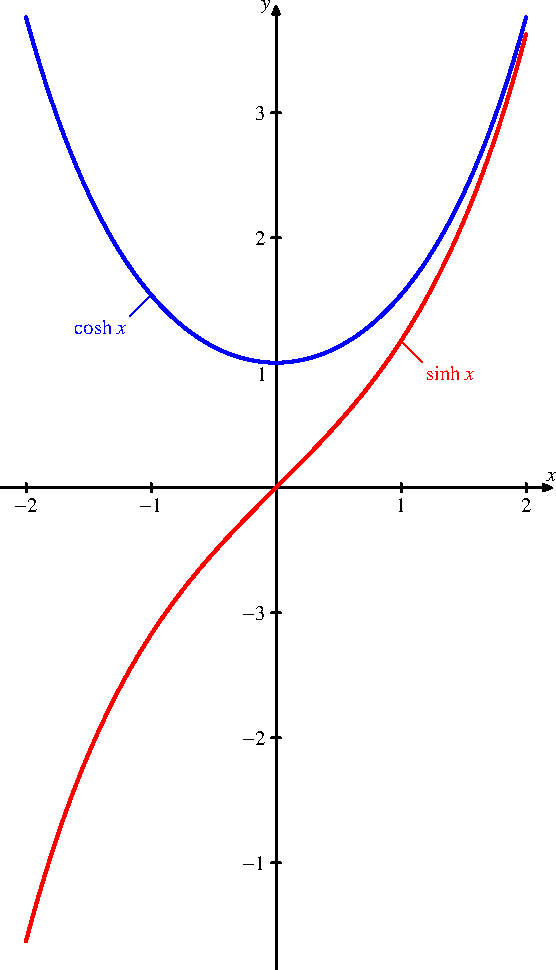
\includegraphics{chapters/mp/hf-1.pdf}
\caption{Graphen der Funktionen $x\mapsto\cosh x$ (blau)
und $x\mapsto\sinh x$ (rot)
\label{hyp:graphen}}
\end{figure}
Die hyperbolischen Funktionen sind durch
\begin{equation}
\sinh x =\frac{e^x-e^{-x}}2
\qquad\text{und}\qquad
\cosh x = \frac{e^x+e^{-x}}2
\label{skript:sinh:definition}
\end{equation}
definiert.
\index{hyperbolische Funktion}
\index{sinh}
\index{cosh}
Abbildung~\ref{hyp:graphen} zeigt die Graphen der beiden Funktionen.
Auf den ersten Blick haben diese Definitionen nichts mit den bekannten
trigonometrischen Funktionen zu tun, die Namen sinus hyperbolicus f"ur
$\sinh$ und cosinus hyperbolicus f"ur $\cosh$ scheinen ungerechtfertigt.

Wie bei den trigonometrischen Funktionen kann man auch die hyperbolische
Tangensfunktion 
\begin{equation}
\tanh x
=
\frac{\sinh x}{\cosh x}
=
\frac{e^x - e^{-x}}{e^x + e^{-x}}
\label{skript:sinh:tanh}
\end{equation}
definieren.

\subsection{Komplexe Definition der trigonometrischen Funktionen}
Aus der Euler-Formel
\[
e^{it}=\cos t+i\sin t
\]
l"asst sich auch eine Definition der trigonometrischen Funktionen
ableiten. Dazu wendet man die Euler-Formel auf $t$ und $-t$ an:
\begin{align*}
\cos t+i\sin t&=e^{it}\\
\cos t-i\sin t&=e^{-it}
\end{align*}
Dieses Gleichungssystem kann man mit der Additionsmethode nach den
Funktionen $\cos t$ und $\sin t$ aufl"osen. Man findet:
\[
\begin{aligned}
\cos t
&=
\frac{e^{it}+e^{-it}}2
&
&\text{und}
&
\sin t
&=
\frac{e^{it}-e^{-it}}{2i}.
\end{aligned}
\]
Die trigonometrischen Funktionen k"onnen also auf eine Art definiert werden,
die der Definition der hyperbolischen Funktionen v"ollig analog ist.
Der einzige Unterschied ist ein Faktor $i$ hie und da.
Wir erwarten daher, dass die hyperbolischen Funktionen Eigenschaften
haben, die den Eigenschaften der trigonometrischen Funktionen v"ollig
analog sind.
Mehr als ein ver"andertes Vorzeichen hie und da erwarten wir nicht.


\subsection{Geometrie}
Die trigonometrischen Funktionen entstanden aus dem Bed"urfnis, 
rechtwinklige Dreiecke berechnen zu k"onnen.
Abstrahiert man diese bis auf "Ahnlichkeit, geht es nur noch um rechtwinklige
Dreiecke, die mindestens eine Seite der L"ange $1$ haben.
Diese kann man auf die gewohnte Art am Einheitskreis illustrieren.
Die Beziehung 
\[
\sin^2t+\cos^2t=1
\]
f"ur die trigonometrischen Funktionen erlauben dann, den Einheitskreis als
\[
t\mapsto (\cos t,\sin t)
\]
zu parametrisieren.

Die hyperbolischen Funktionen parametrisieren in der Form
\[
t\mapsto (\cosh t, \sinh t)
\]
nat"urlich auch eine Kurve in der Ebene.
Um herauszufinden, welcher Kurve das sein k"onnte, berechnen wir die 
Quadrate der hyperbolischen Funktionen:
\begin{align}
\sinh^2 t&=\frac14(e^{2t}-2+e^{-2t}),
\\
\cosh^2 t&=\frac14(e^{2t}+2+e^{-2t}).
\label{hyp:definition}
\end{align}
Sie stimmen bis auf den mittleren Term "uberein.
Die Differenz ist 
\[
\cosh^2t - \sinh^2t=1,
\]
die hyperbolischen Funktionen $x=\cosh t$ und $y=\sinh t$
beschreiben also eine Kurve mit der Gleichung
\[
x^2-y^2=1.
\]
Dies ist eine Hyperbel mit Asymptoten $y=\pm x$. Damit ist die
Bezeichnung als hyperbolische Funktionen gerechtfertigt.

\subsection{Additionstheoreme}
Gibt es auch ein Additionstheorem f"ur die hyperbolischen Funktionen?
Wenn die Analogie zu den trigonometrischen Funktionen durchf"uhrbar ist,
dann m"ussten die Additionstheoreme ungef"ahr die Form
\begin{equation}
\begin{aligned}
\sinh(a+b)&=\sinh a\cosh b + \cosh a\sinh b,\\
\cosh(a+b)&=\cosh a\cosh b - \sinh a\sinh b
\end{aligned}
\label{skript:sinh:additionstheorem:prelim}
\end{equation}
haben, mit einem abweichenden Vorzeichen hie und da.
Um dies nachzupr"ufen, verwenden wir die Definition und rechnen
\begin{align*}
\sinh a\cosh b + \cosh b\sinh b
&=
\frac14(e^a-e^{-a})(e^b+e^{-b})
+
\frac14(e^a+e^{-a})(e^b-e^{-b})
\\
&=\frac14(e^{a+b}+e^{a-b}-e^{-a+b}-e^{-a-b} + e^{a+b}-e^{a-b}+e^{-a+b}-e^{-a-b})
\\
&=
\frac14(2e^{a+b}-2e^{-a-b})
=
\frac12(e^{a+b}-e^{-a-b})=\sinh(a+b),
\\
\cosh a\cosh b-\sinh a\sinh b
&=
\frac14(e^a+e^{-a})(e^b+e^{-b})
-
\frac14(e^a-e^{-a})(e^b-e^{-b})
\\
&=
\frac14(e^{a+b}+e^{a-b}+e^{-a+b}+e^{-a-b})
-
\frac14(e^{a+b}-e^{a-b}-e^{-a+b}+e^{-a-b})
\\
&=
\frac14(2e^{a-b}+2e^{-a+b})
=
\frac12(e^{a-b}+e^{-a+b})=\cosh(a-b)
\end{align*}
aus.
Die Vermutung betreffend der korrekten Form der Additionstheoreme
war also richtig im Falle von $\sinh(a+b)$, f"ur $\cosh(a+b)$ muss
allerdings ein Vorzeichen gewechselt werden.
Die korrekte Form der Additionstheoreme ist
\begin{equation}
\begin{aligned}
\sinh(a\pm b)&=\sinh a\cosh b \pm \cosh a\sinh b,\\
\cosh(a\pm b)&=\cosh a\cosh b \pm \sinh a\sinh b.
\end{aligned}
\label{skript:sinh:additionstheorem}
\end{equation}
Man kann daraus auch ein Additionstheorem für die hyperbolische
Tangens-Funktion ableiten:
\begin{equation}
\tanh(a\pm b) = \frac{\tanh a \pm \tanh b}{1\pm\tanh a\tanh b}.
\label{skript:sinh:addtanh}
\end{equation}

\subsection{Gegenseitige Abhängigkeit%
\label{skript:sinh:section:abh}}
In der Goniometrie lernt man, dass man eine beliebige trigonometrische
Funktion durch jede beliebige andere Funktion ausdrücken kann.
Dies ist auch möglich für hyperbolische Funktionen.
\[
\begin{tabular}{>{$\displaystyle}c<{$}|>{$\displaystyle}c<{$}>{$\displaystyle}c<{$}>{$\displaystyle}c<{$}}
&\sinh x&\cosh x & \tanh x
\\
\hline
\sinh x=\mathstrut
&\sinh x
	&\operatorname{sgn}x\sqrt{\cosh^2x-1}
		&\frac{\tanh x}{\sqrt{1-\tanh^2 x}}
\\
\cosh x=\mathstrut
&\sqrt{1+\sinh^2 x}
	&\cosh x
		&\frac1{\sqrt{1-\tanh^2 x}}
\\
\tanh x=\mathstrut
&\frac{\sinh x}{\sqrt{1+\sinh^2 x}}
	&\operatorname{sgn}x\frac{\sqrt{\cosh^2 x - 1}}{\cosh x}
		&\tanh x
\end{tabular}
\]

\subsection{Ableitungen}
In der Analysis lernt man, die Ableitungen der trigonometrischen Funktionen
aus den Additionstheoremen abzuleiten.
Da die Additionstheoreme der hyperbolischen Funktionen mit den 
Additionstheoremen bis auf ein Vorzeichen "ubereinstimmen, sollten
auch die Ableitungsregeln bis auf ein Vorzeichen mit den Ableitungsregeln
der trigonometrischen Funktionen "ubereinstimmen. 
Nat"urlich k"onnen wir aus der Definition (\ref{hyp:definition}) die
Ableitungen auch direkt berechnen:
\begin{align*}
\frac{d}{dx}\cosh x
&=
\frac12\frac{d}{dx}(e^x+e^{-x})
=
\frac12(e^x-e^{-x})=\sinh x
\\
\frac{d}{dx}\sinh x
&=
\frac12\frac{d}{dx}(e^x-e^{-x})
=
\frac12(e^x+e^{-x})=\cosh x
\end{align*}
Die Ableitungen sind also sogar noch ein bisschen einfacher, da sie sich
schon ab der zweiten Ableitung wiederholen.
Die zweiten Ableitungen sind bereits wieder die urspr"unglichen Funktionen
\begin{align*}
\sinh''x&=\sinh x
&
\cosh''x&=\cosh x.
\end{align*}

\subsection{Werte f"ur Argument 0}
Die Werte der trigonometrischen Funktionen und ihrer ersten Ableitungen
im Nullpunkt und die entsprechenden Werte f"ur die hyperbolischen
Funktionen sind ebenfalls v"ollig analog:
\begin{center}
\begin{tabular}{|l|>{$}c<{$}>{$}c<{$}|>{$}c<{$}>{$}c<{$}|}
\hline
Wert f"ur $x=0$ von&\sin x&\cos x&\sinh x&\cosh x\\
\hline
Funktion           &  0   &  1   &   0   &   1   \\
Ableitung          &  1   &  0   &   1   &   0   \\
\hline
\end{tabular}
\end{center}

\subsection{L"osung von Differentialgleichungen}
Die Werte f"ur Argument $0$ sind genau die Eigenschaften,
welche die Erf"ullung der Anfangsbedingung
einer Differentialgleichung so einfach gemacht haben.
Die Differentialgleichung 
\[
y''-k^2y=0
\]
mit Anfangsbedingungen
\[
y(0)=y_0\qquad\text{und}\qquad y'(0)=v_0
\]
hat die L"osung
\[
y(x)=y_0\cosh kx +\frac{v_0}{k}\sinh kx,
\]
in v"olliger Analogie zu (\ref{hyp:loesung}).

